\documentclass[12pt,letterpaper]{article}
\usepackage[margin=15mm,top=19mm,bottom=18mm,headheight=15pt,headsep=5mm]{geometry}
\usepackage[T1]{fontenc}
\usepackage{helvet}
\renewcommand{\familydefault}{\sfdefault}
\usepackage{tikz}
\usepackage{fancyhdr}
\usepackage{array}
\usepackage{amsmath}
\definecolor{polygonline}{rgb}{0.12,0.16,0.20}
\pagestyle{fancy}
\fancyhf{}
\renewcommand{\headrulewidth}{0pt}
\renewcommand{\footrulewidth}{0pt}
\newcommand{\Band}{Grades 3--5}
\fancyhead[L]{\small Week 57 / Area from dots / \Band}
\fancyfoot[L]{\footnotesize Bellingham Math Circle / Week 57 / N57-S-final-v3}
\fancyfoot[R]{\footnotesize\thepage}
\setlength{\parindent}{0pt}
\setlength{\parskip}{3mm}
\renewcommand{\arraystretch}{1.6}
\newcommand{\Problem}[2]{\textbf{Problem #1:} #2\par}
\newcommand{\BlankBoard}[2]{%
\begin{tikzpicture}[x=20mm,y=20mm]
\path[use as bounding box] (-.12,-.12) rectangle (#1+.12,#2+.12);
\foreach \x in {0,...,#1} \foreach \y in {0,...,#2}
  \fill (\x,\y) circle[radius=.55mm];
\end{tikzpicture}}
\newcommand{\Record}{\(I=\)\rule{12mm}{.3pt}\quad\(B=\)\rule{12mm}{.3pt}\quad area\(=\)\rule{12mm}{.3pt}}
\newcommand{\PairFigures}[2]{%
\begin{center}\begin{minipage}[t]{.48\textwidth}\centering\Figure{#1}\end{minipage}\hfill%
\begin{minipage}[t]{.48\textwidth}\centering\Figure{#2}\end{minipage}\end{center}}
% The figure macros (\Figure{name}) come first in the body, from figures.py.
\begin{document}

\newcommand{\Figure}[1]{\csname figure#1\endcsname}
\expandafter\def\csname figurearea-input\endcsname{%
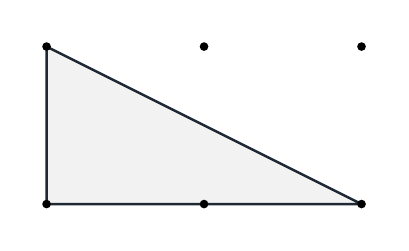
\begin{tikzpicture}[x=20mm,y=20mm]
\path[use as bounding box] (-.12,-.12) rectangle (2.12,1.12);
\path[fill=black!5] (0,0) -- (2,0) -- (0,1) -- cycle;
\draw[draw=polygonline,line width=.9pt,line join=round] (0,0) -- (2,0) -- (0,1) -- cycle;
\fill[black] (0,0) circle[radius=.55mm];
\fill[black] (0,1) circle[radius=.55mm];
\fill[black] (1,0) circle[radius=.55mm];
\fill[black] (1,1) circle[radius=.55mm];
\fill[black] (2,0) circle[radius=.55mm];
\fill[black] (2,1) circle[radius=.55mm];
\end{tikzpicture}
}
\expandafter\def\csname figurearea-joined\endcsname{%
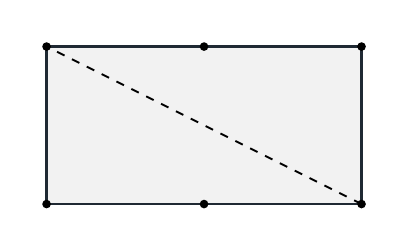
\begin{tikzpicture}[x=20mm,y=20mm]
\path[use as bounding box] (-.12,-.12) rectangle (2.12,1.12);
\path[fill=black!5] (0,0) -- (2,0) -- (2,1) -- (0,1) -- cycle;
\draw[draw=polygonline,line width=.9pt,line join=round] (0,0) -- (2,0) -- (2,1) -- (0,1) -- cycle;
\draw[dashed,line width=.7pt] (2,0) -- (0,1);
\fill[black] (0,0) circle[radius=.55mm];
\fill[black] (0,1) circle[radius=.55mm];
\fill[black] (1,0) circle[radius=.55mm];
\fill[black] (1,1) circle[radius=.55mm];
\fill[black] (2,0) circle[radius=.55mm];
\fill[black] (2,1) circle[radius=.55mm];
\end{tikzpicture}
}
\expandafter\def\csname figurearea-rectangle\endcsname{%
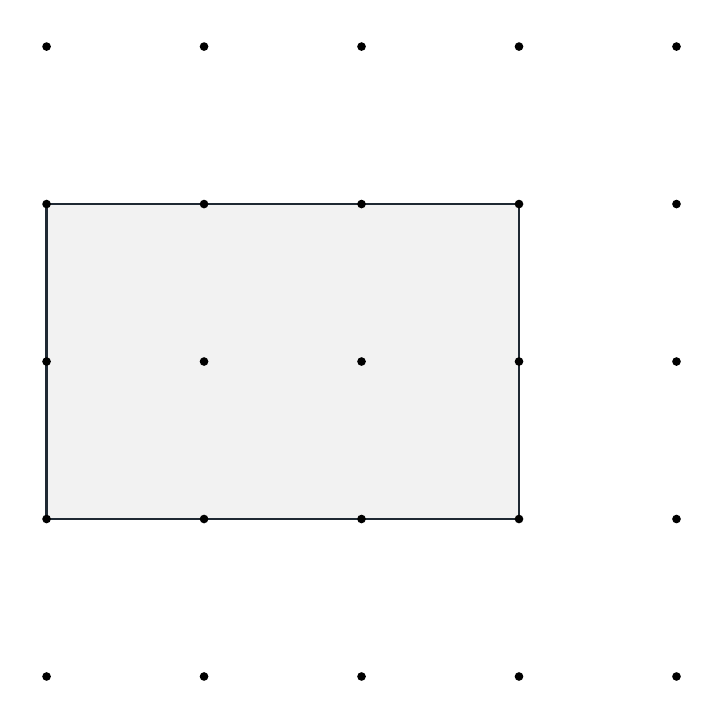
\begin{tikzpicture}[x=20mm,y=20mm]
\path[use as bounding box] (-.12,-.12) rectangle (4.12,4.12);
\path[fill=black!5] (0,1) -- (3,1) -- (3,3) -- (0,3) -- cycle;
\draw[draw=polygonline,line width=.9pt,line join=round] (0,1) -- (3,1) -- (3,3) -- (0,3) -- cycle;
\fill[black] (0,0) circle[radius=.55mm];
\fill[black] (0,1) circle[radius=.55mm];
\fill[black] (0,2) circle[radius=.55mm];
\fill[black] (0,3) circle[radius=.55mm];
\fill[black] (0,4) circle[radius=.55mm];
\fill[black] (1,0) circle[radius=.55mm];
\fill[black] (1,1) circle[radius=.55mm];
\fill[black] (1,2) circle[radius=.55mm];
\fill[black] (1,3) circle[radius=.55mm];
\fill[black] (1,4) circle[radius=.55mm];
\fill[black] (2,0) circle[radius=.55mm];
\fill[black] (2,1) circle[radius=.55mm];
\fill[black] (2,2) circle[radius=.55mm];
\fill[black] (2,3) circle[radius=.55mm];
\fill[black] (2,4) circle[radius=.55mm];
\fill[black] (3,0) circle[radius=.55mm];
\fill[black] (3,1) circle[radius=.55mm];
\fill[black] (3,2) circle[radius=.55mm];
\fill[black] (3,3) circle[radius=.55mm];
\fill[black] (3,4) circle[radius=.55mm];
\fill[black] (4,0) circle[radius=.55mm];
\fill[black] (4,1) circle[radius=.55mm];
\fill[black] (4,2) circle[radius=.55mm];
\fill[black] (4,3) circle[radius=.55mm];
\fill[black] (4,4) circle[radius=.55mm];
\end{tikzpicture}
}
\expandafter\def\csname figurearea-slanted\endcsname{%
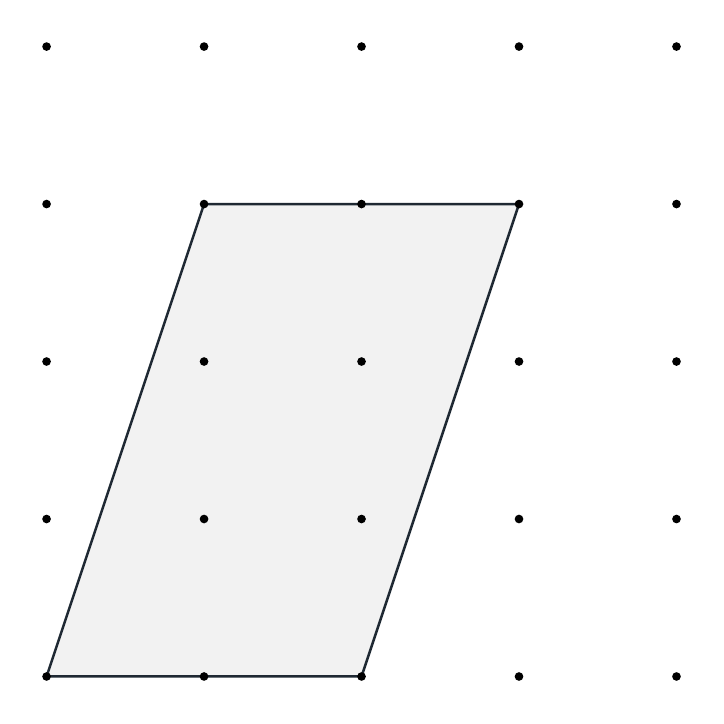
\begin{tikzpicture}[x=20mm,y=20mm]
\path[use as bounding box] (-.12,-.12) rectangle (4.12,4.12);
\path[fill=black!5] (0,0) -- (2,0) -- (3,3) -- (1,3) -- cycle;
\draw[draw=polygonline,line width=.9pt,line join=round] (0,0) -- (2,0) -- (3,3) -- (1,3) -- cycle;
\fill[black] (0,0) circle[radius=.55mm];
\fill[black] (0,1) circle[radius=.55mm];
\fill[black] (0,2) circle[radius=.55mm];
\fill[black] (0,3) circle[radius=.55mm];
\fill[black] (0,4) circle[radius=.55mm];
\fill[black] (1,0) circle[radius=.55mm];
\fill[black] (1,1) circle[radius=.55mm];
\fill[black] (1,2) circle[radius=.55mm];
\fill[black] (1,3) circle[radius=.55mm];
\fill[black] (1,4) circle[radius=.55mm];
\fill[black] (2,0) circle[radius=.55mm];
\fill[black] (2,1) circle[radius=.55mm];
\fill[black] (2,2) circle[radius=.55mm];
\fill[black] (2,3) circle[radius=.55mm];
\fill[black] (2,4) circle[radius=.55mm];
\fill[black] (3,0) circle[radius=.55mm];
\fill[black] (3,1) circle[radius=.55mm];
\fill[black] (3,2) circle[radius=.55mm];
\fill[black] (3,3) circle[radius=.55mm];
\fill[black] (3,4) circle[radius=.55mm];
\fill[black] (4,0) circle[radius=.55mm];
\fill[black] (4,1) circle[radius=.55mm];
\fill[black] (4,2) circle[radius=.55mm];
\fill[black] (4,3) circle[radius=.55mm];
\fill[black] (4,4) circle[radius=.55mm];
\end{tikzpicture}
}
\expandafter\def\csname figurecount-input\endcsname{%
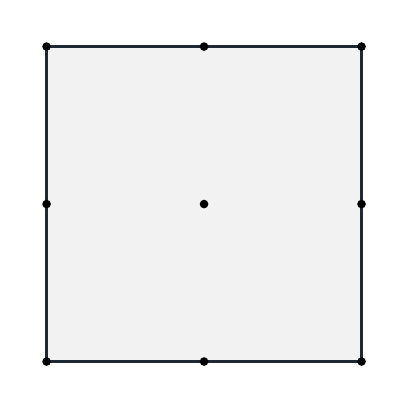
\begin{tikzpicture}[x=20mm,y=20mm]
\path[use as bounding box] (-.12,-.12) rectangle (2.12,2.12);
\path[fill=black!5] (0,0) -- (2,0) -- (2,2) -- (0,2) -- cycle;
\draw[draw=polygonline,line width=.9pt,line join=round] (0,0) -- (2,0) -- (2,2) -- (0,2) -- cycle;
\fill[black] (0,0) circle[radius=.55mm];
\fill[black] (0,1) circle[radius=.55mm];
\fill[black] (0,2) circle[radius=.55mm];
\fill[black] (1,0) circle[radius=.55mm];
\fill[black] (1,1) circle[radius=.55mm];
\fill[black] (1,2) circle[radius=.55mm];
\fill[black] (2,0) circle[radius=.55mm];
\fill[black] (2,1) circle[radius=.55mm];
\fill[black] (2,2) circle[radius=.55mm];
\end{tikzpicture}
}
\expandafter\def\csname figurecount-marked\endcsname{%
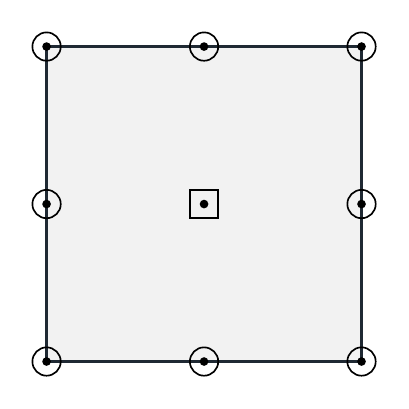
\begin{tikzpicture}[x=20mm,y=20mm]
\path[use as bounding box] (-.12,-.12) rectangle (2.12,2.12);
\path[fill=black!5] (0,0) -- (2,0) -- (2,2) -- (0,2) -- cycle;
\draw[draw=polygonline,line width=.9pt,line join=round] (0,0) -- (2,0) -- (2,2) -- (0,2) -- cycle;
\fill[black] (0,0) circle[radius=.55mm];
\draw[line width=.6pt] (0,0) circle[radius=1.8mm];
\fill[black] (0,1) circle[radius=.55mm];
\draw[line width=.6pt] (0,1) circle[radius=1.8mm];
\fill[black] (0,2) circle[radius=.55mm];
\draw[line width=.6pt] (0,2) circle[radius=1.8mm];
\fill[black] (1,0) circle[radius=.55mm];
\draw[line width=.6pt] (1,0) circle[radius=1.8mm];
\fill[black] (1,1) circle[radius=.55mm];
\draw[line width=.6pt] (0.91,0.91) rectangle (1.09,1.09);
\fill[black] (1,2) circle[radius=.55mm];
\draw[line width=.6pt] (1,2) circle[radius=1.8mm];
\fill[black] (2,0) circle[radius=.55mm];
\draw[line width=.6pt] (2,0) circle[radius=1.8mm];
\fill[black] (2,1) circle[radius=.55mm];
\draw[line width=.6pt] (2,1) circle[radius=1.8mm];
\fill[black] (2,2) circle[radius=.55mm];
\draw[line width=.6pt] (2,2) circle[radius=1.8mm];
\end{tikzpicture}
}
\expandafter\def\csname figurecount-L\endcsname{%
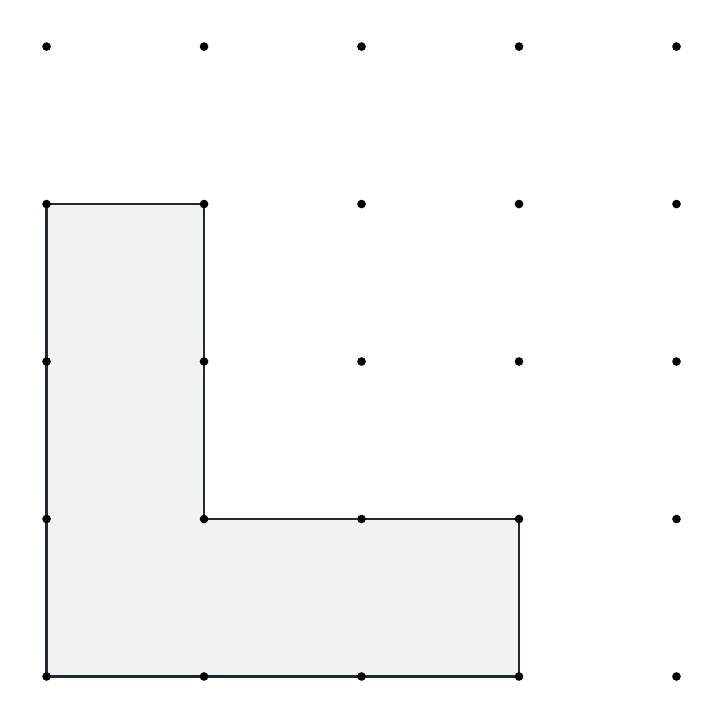
\begin{tikzpicture}[x=20mm,y=20mm]
\path[use as bounding box] (-.12,-.12) rectangle (4.12,4.12);
\path[fill=black!5] (0,0) -- (3,0) -- (3,1) -- (1,1) -- (1,3) -- (0,3) -- cycle;
\draw[draw=polygonline,line width=.9pt,line join=round] (0,0) -- (3,0) -- (3,1) -- (1,1) -- (1,3) -- (0,3) -- cycle;
\fill[black] (0,0) circle[radius=.55mm];
\fill[black] (0,1) circle[radius=.55mm];
\fill[black] (0,2) circle[radius=.55mm];
\fill[black] (0,3) circle[radius=.55mm];
\fill[black] (0,4) circle[radius=.55mm];
\fill[black] (1,0) circle[radius=.55mm];
\fill[black] (1,1) circle[radius=.55mm];
\fill[black] (1,2) circle[radius=.55mm];
\fill[black] (1,3) circle[radius=.55mm];
\fill[black] (1,4) circle[radius=.55mm];
\fill[black] (2,0) circle[radius=.55mm];
\fill[black] (2,1) circle[radius=.55mm];
\fill[black] (2,2) circle[radius=.55mm];
\fill[black] (2,3) circle[radius=.55mm];
\fill[black] (2,4) circle[radius=.55mm];
\fill[black] (3,0) circle[radius=.55mm];
\fill[black] (3,1) circle[radius=.55mm];
\fill[black] (3,2) circle[radius=.55mm];
\fill[black] (3,3) circle[radius=.55mm];
\fill[black] (3,4) circle[radius=.55mm];
\fill[black] (4,0) circle[radius=.55mm];
\fill[black] (4,1) circle[radius=.55mm];
\fill[black] (4,2) circle[radius=.55mm];
\fill[black] (4,3) circle[radius=.55mm];
\fill[black] (4,4) circle[radius=.55mm];
\end{tikzpicture}
}
\expandafter\def\csname figurecount-triangle\endcsname{%
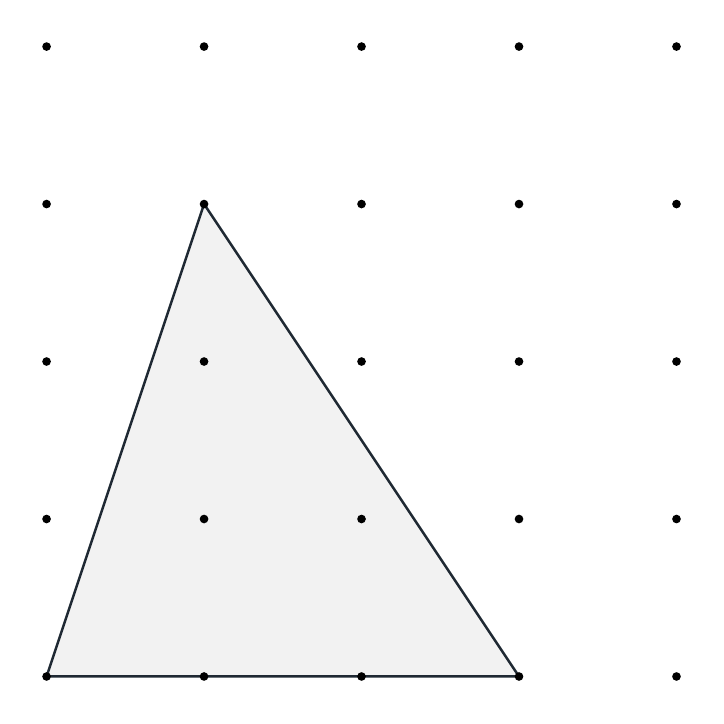
\begin{tikzpicture}[x=20mm,y=20mm]
\path[use as bounding box] (-.12,-.12) rectangle (4.12,4.12);
\path[fill=black!5] (0,0) -- (3,0) -- (1,3) -- cycle;
\draw[draw=polygonline,line width=.9pt,line join=round] (0,0) -- (3,0) -- (1,3) -- cycle;
\fill[black] (0,0) circle[radius=.55mm];
\fill[black] (0,1) circle[radius=.55mm];
\fill[black] (0,2) circle[radius=.55mm];
\fill[black] (0,3) circle[radius=.55mm];
\fill[black] (0,4) circle[radius=.55mm];
\fill[black] (1,0) circle[radius=.55mm];
\fill[black] (1,1) circle[radius=.55mm];
\fill[black] (1,2) circle[radius=.55mm];
\fill[black] (1,3) circle[radius=.55mm];
\fill[black] (1,4) circle[radius=.55mm];
\fill[black] (2,0) circle[radius=.55mm];
\fill[black] (2,1) circle[radius=.55mm];
\fill[black] (2,2) circle[radius=.55mm];
\fill[black] (2,3) circle[radius=.55mm];
\fill[black] (2,4) circle[radius=.55mm];
\fill[black] (3,0) circle[radius=.55mm];
\fill[black] (3,1) circle[radius=.55mm];
\fill[black] (3,2) circle[radius=.55mm];
\fill[black] (3,3) circle[radius=.55mm];
\fill[black] (3,4) circle[radius=.55mm];
\fill[black] (4,0) circle[radius=.55mm];
\fill[black] (4,1) circle[radius=.55mm];
\fill[black] (4,2) circle[radius=.55mm];
\fill[black] (4,3) circle[radius=.55mm];
\fill[black] (4,4) circle[radius=.55mm];
\end{tikzpicture}
}
\expandafter\def\csname figurejoin-rectangle\endcsname{%
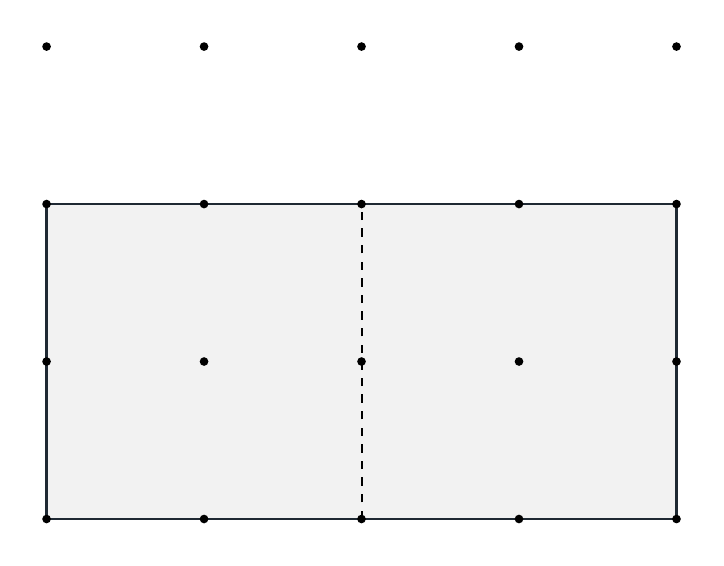
\begin{tikzpicture}[x=20mm,y=20mm]
\path[use as bounding box] (-.12,-.12) rectangle (4.12,3.12);
\path[fill=black!5] (0,0) -- (4,0) -- (4,2) -- (0,2) -- cycle;
\draw[draw=polygonline,line width=.9pt,line join=round] (0,0) -- (4,0) -- (4,2) -- (0,2) -- cycle;
\draw[dashed,line width=.7pt] (2,0) -- (2,2);
\fill[black] (0,0) circle[radius=.55mm];
\fill[black] (0,1) circle[radius=.55mm];
\fill[black] (0,2) circle[radius=.55mm];
\fill[black] (0,3) circle[radius=.55mm];
\fill[black] (1,0) circle[radius=.55mm];
\fill[black] (1,1) circle[radius=.55mm];
\fill[black] (1,2) circle[radius=.55mm];
\fill[black] (1,3) circle[radius=.55mm];
\fill[black] (2,0) circle[radius=.55mm];
\fill[black] (2,1) circle[radius=.55mm];
\fill[black] (2,2) circle[radius=.55mm];
\fill[black] (2,3) circle[radius=.55mm];
\fill[black] (3,0) circle[radius=.55mm];
\fill[black] (3,1) circle[radius=.55mm];
\fill[black] (3,2) circle[radius=.55mm];
\fill[black] (3,3) circle[radius=.55mm];
\fill[black] (4,0) circle[radius=.55mm];
\fill[black] (4,1) circle[radius=.55mm];
\fill[black] (4,2) circle[radius=.55mm];
\fill[black] (4,3) circle[radius=.55mm];
\end{tikzpicture}
}
\expandafter\def\csname figurejoin-slanted\endcsname{%
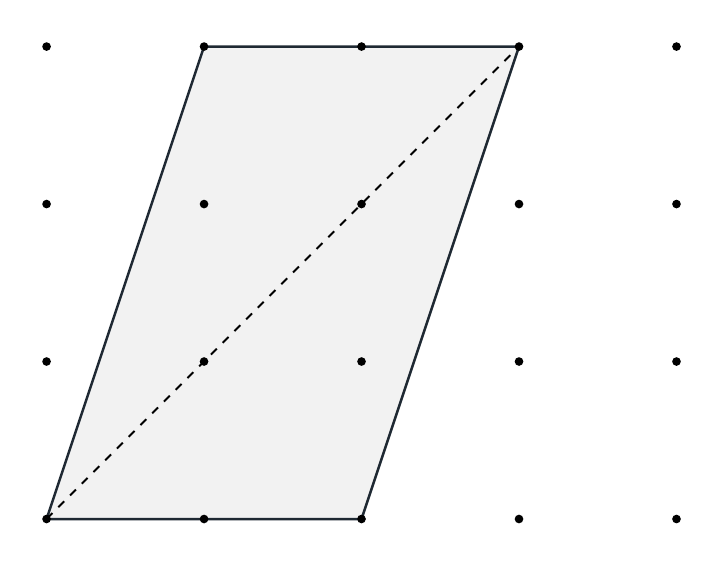
\begin{tikzpicture}[x=20mm,y=20mm]
\path[use as bounding box] (-.12,-.12) rectangle (4.12,3.12);
\path[fill=black!5] (0,0) -- (2,0) -- (3,3) -- (1,3) -- cycle;
\draw[draw=polygonline,line width=.9pt,line join=round] (0,0) -- (2,0) -- (3,3) -- (1,3) -- cycle;
\draw[dashed,line width=.7pt] (0,0) -- (3,3);
\fill[black] (0,0) circle[radius=.55mm];
\fill[black] (0,1) circle[radius=.55mm];
\fill[black] (0,2) circle[radius=.55mm];
\fill[black] (0,3) circle[radius=.55mm];
\fill[black] (1,0) circle[radius=.55mm];
\fill[black] (1,1) circle[radius=.55mm];
\fill[black] (1,2) circle[radius=.55mm];
\fill[black] (1,3) circle[radius=.55mm];
\fill[black] (2,0) circle[radius=.55mm];
\fill[black] (2,1) circle[radius=.55mm];
\fill[black] (2,2) circle[radius=.55mm];
\fill[black] (2,3) circle[radius=.55mm];
\fill[black] (3,0) circle[radius=.55mm];
\fill[black] (3,1) circle[radius=.55mm];
\fill[black] (3,2) circle[radius=.55mm];
\fill[black] (3,3) circle[radius=.55mm];
\fill[black] (4,0) circle[radius=.55mm];
\fill[black] (4,1) circle[radius=.55mm];
\fill[black] (4,2) circle[radius=.55mm];
\fill[black] (4,3) circle[radius=.55mm];
\end{tikzpicture}
}
\expandafter\def\csname figureexplain-triangle\endcsname{%
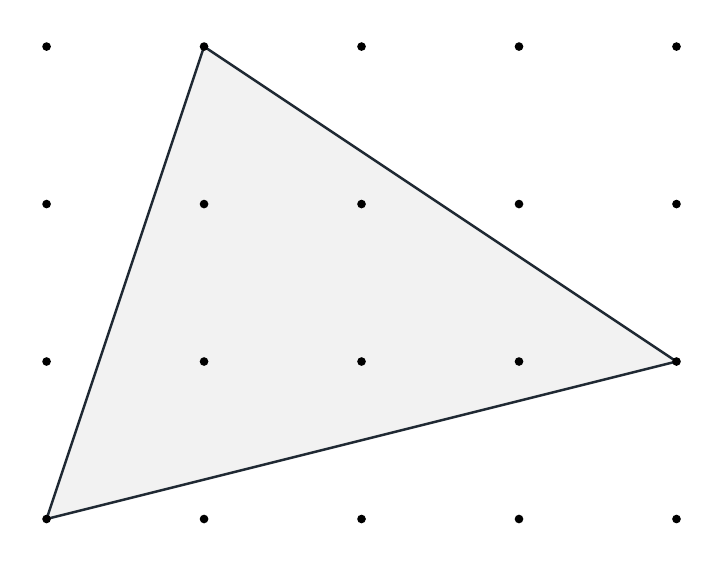
\begin{tikzpicture}[x=20mm,y=20mm]
\path[use as bounding box] (-.12,-.12) rectangle (4.12,3.12);
\path[fill=black!5] (0,0) -- (4,1) -- (1,3) -- cycle;
\draw[draw=polygonline,line width=.9pt,line join=round] (0,0) -- (4,1) -- (1,3) -- cycle;
\fill[black] (0,0) circle[radius=.55mm];
\fill[black] (0,1) circle[radius=.55mm];
\fill[black] (0,2) circle[radius=.55mm];
\fill[black] (0,3) circle[radius=.55mm];
\fill[black] (1,0) circle[radius=.55mm];
\fill[black] (1,1) circle[radius=.55mm];
\fill[black] (1,2) circle[radius=.55mm];
\fill[black] (1,3) circle[radius=.55mm];
\fill[black] (2,0) circle[radius=.55mm];
\fill[black] (2,1) circle[radius=.55mm];
\fill[black] (2,2) circle[radius=.55mm];
\fill[black] (2,3) circle[radius=.55mm];
\fill[black] (3,0) circle[radius=.55mm];
\fill[black] (3,1) circle[radius=.55mm];
\fill[black] (3,2) circle[radius=.55mm];
\fill[black] (3,3) circle[radius=.55mm];
\fill[black] (4,0) circle[radius=.55mm];
\fill[black] (4,1) circle[radius=.55mm];
\fill[black] (4,2) circle[radius=.55mm];
\fill[black] (4,3) circle[radius=.55mm];
\end{tikzpicture}
}
\expandafter\def\csname figureexplain-concave\endcsname{%
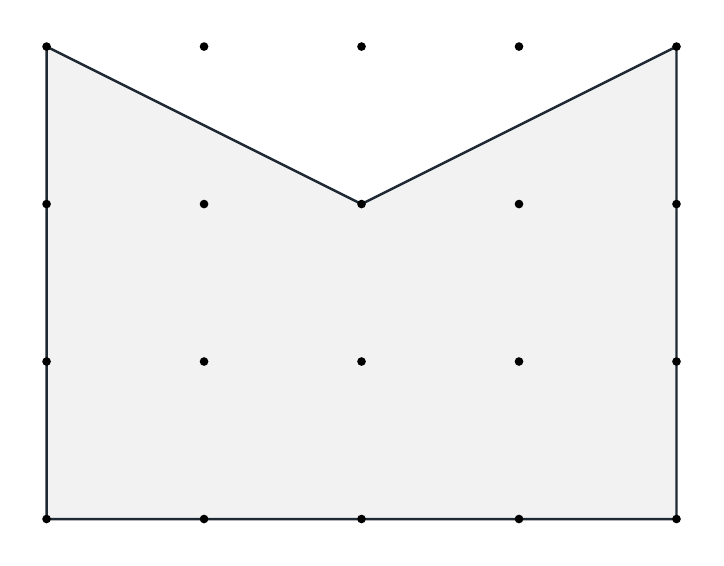
\begin{tikzpicture}[x=20mm,y=20mm]
\path[use as bounding box] (-.12,-.12) rectangle (4.12,3.12);
\path[fill=black!5] (0,0) -- (4,0) -- (4,3) -- (2,2) -- (0,3) -- cycle;
\draw[draw=polygonline,line width=.9pt,line join=round] (0,0) -- (4,0) -- (4,3) -- (2,2) -- (0,3) -- cycle;
\fill[black] (0,0) circle[radius=.55mm];
\fill[black] (0,1) circle[radius=.55mm];
\fill[black] (0,2) circle[radius=.55mm];
\fill[black] (0,3) circle[radius=.55mm];
\fill[black] (1,0) circle[radius=.55mm];
\fill[black] (1,1) circle[radius=.55mm];
\fill[black] (1,2) circle[radius=.55mm];
\fill[black] (1,3) circle[radius=.55mm];
\fill[black] (2,0) circle[radius=.55mm];
\fill[black] (2,1) circle[radius=.55mm];
\fill[black] (2,2) circle[radius=.55mm];
\fill[black] (2,3) circle[radius=.55mm];
\fill[black] (3,0) circle[radius=.55mm];
\fill[black] (3,1) circle[radius=.55mm];
\fill[black] (3,2) circle[radius=.55mm];
\fill[black] (3,3) circle[radius=.55mm];
\fill[black] (4,0) circle[radius=.55mm];
\fill[black] (4,1) circle[radius=.55mm];
\fill[black] (4,2) circle[radius=.55mm];
\fill[black] (4,3) circle[radius=.55mm];
\end{tikzpicture}
}
\expandafter\def\csname figurehole-square\endcsname{%
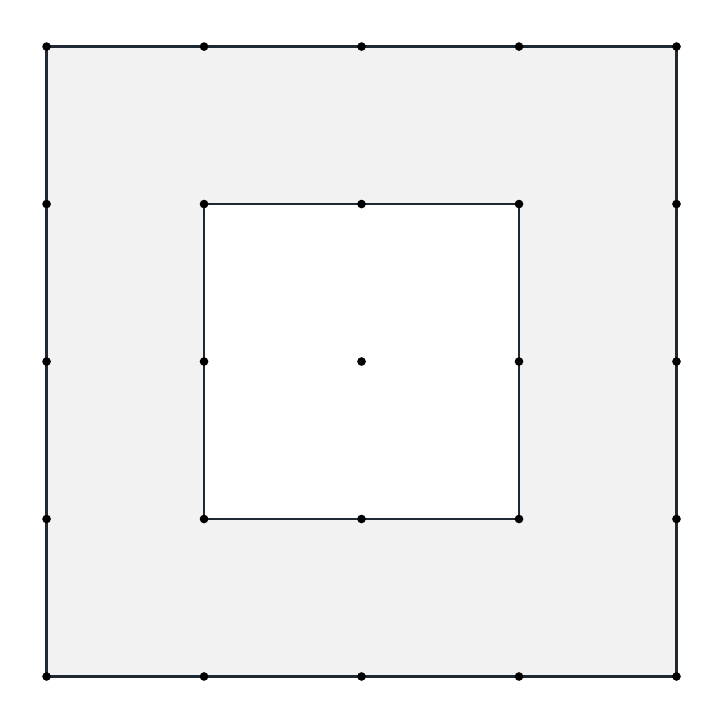
\begin{tikzpicture}[x=20mm,y=20mm]
\path[use as bounding box] (-.12,-.12) rectangle (4.12,4.12);
\path[fill=black!5] (0,0) -- (4,0) -- (4,4) -- (0,4) -- cycle;
\path[fill=white] (1,1) -- (3,1) -- (3,3) -- (1,3) -- cycle;
\draw[draw=polygonline,line width=.9pt,line join=round] (0,0) -- (4,0) -- (4,4) -- (0,4) -- cycle;
\draw[draw=polygonline,line width=.9pt,line join=round] (1,1) -- (3,1) -- (3,3) -- (1,3) -- cycle;
\fill[black] (0,0) circle[radius=.55mm];
\fill[black] (0,1) circle[radius=.55mm];
\fill[black] (0,2) circle[radius=.55mm];
\fill[black] (0,3) circle[radius=.55mm];
\fill[black] (0,4) circle[radius=.55mm];
\fill[black] (1,0) circle[radius=.55mm];
\fill[black] (1,1) circle[radius=.55mm];
\fill[black] (1,2) circle[radius=.55mm];
\fill[black] (1,3) circle[radius=.55mm];
\fill[black] (1,4) circle[radius=.55mm];
\fill[black] (2,0) circle[radius=.55mm];
\fill[black] (2,1) circle[radius=.55mm];
\fill[black] (2,2) circle[radius=.55mm];
\fill[black] (2,3) circle[radius=.55mm];
\fill[black] (2,4) circle[radius=.55mm];
\fill[black] (3,0) circle[radius=.55mm];
\fill[black] (3,1) circle[radius=.55mm];
\fill[black] (3,2) circle[radius=.55mm];
\fill[black] (3,3) circle[radius=.55mm];
\fill[black] (3,4) circle[radius=.55mm];
\fill[black] (4,0) circle[radius=.55mm];
\fill[black] (4,1) circle[radius=.55mm];
\fill[black] (4,2) circle[radius=.55mm];
\fill[black] (4,3) circle[radius=.55mm];
\fill[black] (4,4) circle[radius=.55mm];
\end{tikzpicture}
}

Join dots with straight sides to make one closed outline. Sides cannot cross or touch except at neighboring corners. The area of one grid square is 1. Find or check areas with pieces, cuts or copies.

\begin{center}
\begin{minipage}[t]{.31\textwidth}\centering
Input\par\Figure{area-input}
\end{minipage}\hfill
\begin{minipage}[t]{.36\textwidth}\centering
Two copies joined\par\Figure{area-joined}
\end{minipage}\hfill
\begin{minipage}[t]{.27\textwidth}\centering
Output\par
\vspace{3mm}
Rectangle area: 2\par
One copy's area: 1
\end{minipage}
\end{center}

\Problem{1}{Find the exact area of each shape.}

\PairFigures{area-rectangle}{area-slanted}
\begin{center}
\begin{minipage}{.48\textwidth}\centering area\(=\)\rule{22mm}{.3pt}\end{minipage}\hfill
\begin{minipage}{.48\textwidth}\centering area\(=\)\rule{22mm}{.3pt}\end{minipage}
\end{center}
\vfill

\newpage

\(I\) counts dots strictly inside. \(B\) counts every dot on the outline, including dots between corners. Count each dot once.
\begin{center}
\begin{minipage}[t]{.31\textwidth}\centering
Input\par\Figure{count-input}
\end{minipage}\hfill
\begin{minipage}[t]{.36\textwidth}\centering
Marked dots\par\Figure{count-marked}\par
\small circle: boundary\par box: inside
\end{minipage}\hfill
\begin{minipage}[t]{.27\textwidth}\centering
Output\par\vspace{6mm}
\(I=1\)\par\(B=8\)\par area\(=4\)
\end{minipage}
\end{center}

\Problem{2}{For each shape, mark the dots you count and make an \(I,B,\text{area}\) record.}

\PairFigures{count-L}{count-triangle}
\begin{center}
\begin{minipage}{.48\textwidth}\centering\Record\end{minipage}\hfill
\begin{minipage}{.48\textwidth}\centering\Record\end{minipage}
\end{center}
\vfill

\newpage

\Problem{3}{Make a triangle and a four-sided shape, each with \(I=2\) and \(B=6\). Find their areas.}

\begin{center}
\BlankBoard{4}{4}\par\Record\par\vspace{20mm}
\BlankBoard{4}{4}\par\Record
\end{center}
\vfill

\newpage

\Problem{4}{Find a rule that predicts area from \(I\) and \(B\). Use all your records. Draw a new shape that could defeat your rule.}

\begin{center}\BlankBoard{6}{6}\par\Record\end{center}
\vfill

\newpage

\Problem{5}{Pick's rule for the allowed polygons is
\[\text{area}= I + (\text{half of }B) - 1.\]
Make shapes of area 6 with as many different \((I,B)\) records as you can.}

\begin{center}\BlankBoard{6}{6}\end{center}
\vfill

\newpage

\Problem{6}{Each dashed seam cuts a shape into two pieces. Make an \(I,B,\text{area}\) record for each piece and for the whole shape. What changes when the seam disappears?}

\PairFigures{join-rectangle}{join-slanted}
\begin{center}
\begin{minipage}[t]{.48\textwidth}
Left piece: \par\Record\par
Right piece: \par\Record\par
Whole: \par\Record
\end{minipage}\hfill
\begin{minipage}[t]{.48\textwidth}
Lower piece: \par\Record\par
Upper piece: \par\Record\par
Whole: \par\Record
\end{minipage}
\end{center}
\vfill

\newpage

\renewcommand{\Band}{Grades 4--5}

\Problem{7}{Join two allowed polygons along one whole side. They must meet only on that side, and the joined shape must obey the shared rules. Explain why the two values \(I+(\text{half of }B)-1\) add to the value for the whole. Your explanation must work however many dots lie on the shared side.}

\begin{center}\BlankBoard{6}{6}\end{center}
\vfill

\newpage

\Problem{8}{Explain why Pick's rule works for every allowed polygon, including these two.}

\PairFigures{explain-triangle}{explain-concave}
\vfill

\newpage

Keep each hole inside the outer outline. All boundary loops must stay separate, with straight sides and corners on dots. Count dots on all outlines in \(B\); dots in a hole do not count in \(I\).

\Problem{9}{The shaded shape has a square hole. Find its area, \(I\) and \(B\). How must Pick's rule change when there is one hole? Test your change on another shape with one hole.}

\begin{center}\Figure{hole-square}\par\Record\end{center}
\begin{center}\BlankBoard{6}{3}\end{center}
\vfill

\newpage

\Problem{10}{Make a connected shape with two holes. Find area without using dot counts. Then find a dot-count rule for a connected shape with any number of holes.}

\begin{center}\BlankBoard{6}{6}\par\Record\end{center}
\vfill
\end{document}
